\section{Experiments}

In this section we present empirical results based on our
implementation the \gwin~ algorithm from the previous section (see appendix for
the python code).
As proved in the previous section, the algorithm should succeed with high
probability when $n \sim \Omega(m^2)$ so we tested values for $n$ ranging between
$n = m^{1.5}$ to $m^{2.5}$ for each $m$ between 5 and 50.
For $m \in [50,100]$ we ran experiments for $n = m^{2.1}$ to $m^{2.5}$
Note that the experimental values for $m$ were not evenly spaced apart.
Each pair of $n,m$ was run for 100 trials, each trial consisting of generating
an election uniformly at random, picking a random candidate to test, and running \gwin~ on that
instance.
A success was when \gwin~returned ``definitely'', as in it was self-knowingly correct.

At 100 candidates, the 100 trials took 9 hours, while at 5 candidates, the trials
took about 3 minutes.


\begin{figure}[hbt!]\centering
    \subfloat{
    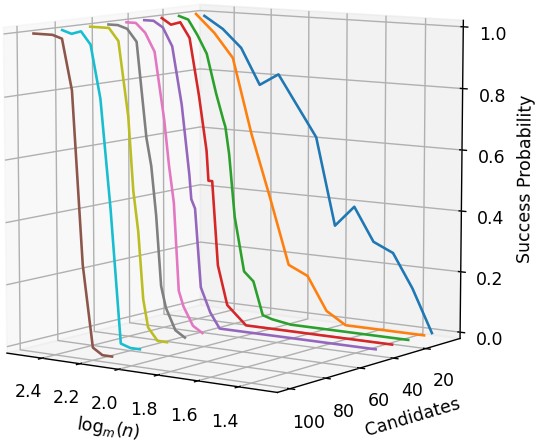
\includegraphics[width=0.45\linewidth]{gwinNoErr.png}}\hfill
    \subfloat{
    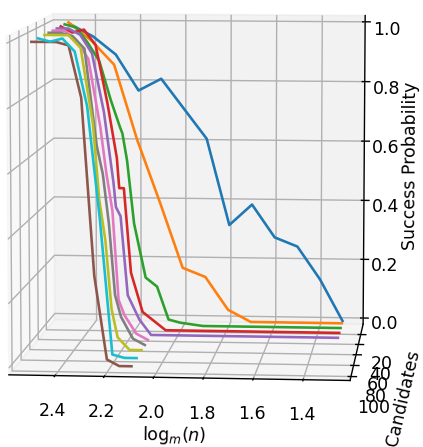
\includegraphics[width=0.45\linewidth]{view2.png}}
    \caption{3D line plot showing the success probability of the
    \gwin~algorithm. Each line color corresponds to a particular
    number of candidates. 100 trials were run for each pair of $n,m$.
    Error bars were omitted to not clutter the graph. For reference they
    are at most $\pm 0.08$.}
    \label{fig:exp}
\end{figure}

Figure \ref{fig:exp} confirms the theoretical result that \gwin~succeeds with
high probability when $n \sim \Omega(m^2)$.
Though the figure shows close to 1 probability of success when $n \geq m^{2.3}$,
this can be explained by the other less significant terms in the polynomial which
are showing a large effect at low values of $m$.
Due to computational constraints, it was only feasible to experiment with up to
100 candidates.
Observe also that when $m \leq 30$, the less significant terms have a large effect,
dragging the line towards linear in $\log_m(n)$ (the exponent), as $m$ decreases.




